% ============================================================================
%  Problems: สามเหลี่ยม (Triangles)
%  Ordered from easy (basic) → intermediate.
%  Shared by exercise.tex and answer-key.tex
% ============================================================================

% --- Part 1: พื้นฐาน (Basic) ---
\examsection{ตอนที่ 1: พื้นฐาน — ชนิดและมุมของสามเหลี่ยม}

\problem{
  สามเหลี่ยมมีด้านยาว 5, 5, 8 เซนติเมตร จงจำแนกชนิดของสามเหลี่ยมนี้ตามด้าน
}{
  มีด้านเท่ากัน 2 ด้าน $(5 = 5)$ ดังนั้นเป็น \textbf{สามเหลี่ยมหน้าจั่ว}
}

\problem{
  สามเหลี่ยมมีมุม $30^\circ$, $60^\circ$, $90^\circ$ จงจำแนกชนิดของสามเหลี่ยมนี้ตามมุม
}{
  มีมุม $90^\circ$ หนึ่งมุม ดังนั้นเป็น \textbf{สามเหลี่ยมมุมฉาก}
}

\problem{
  สามเหลี่ยมหน้าจั่วมีมุมยอด (vertex angle) $= 40^\circ$
  จงหาขนาดของมุมฐานแต่ละมุม
}{
  มุมฐานเท่ากัน: มุมฐานแต่ละมุม $= \dfrac{180^\circ - 40^\circ}{2}
  = \dfrac{140^\circ}{2} = 70^\circ$
}

\problem{
  สามเหลี่ยมหน้าจั่วมีมุมฐานมุมละ $55^\circ$
  จงหาขนาดของมุมยอด
}{
  มุมยอด $= 180^\circ - 55^\circ - 55^\circ = 70^\circ$
}

% --- Part 2: การประยุกต์ (Intermediate) ---
\examsection{ตอนที่ 2: การประยุกต์ — พีทาโกรัส, ความคล้าย, สามเหลี่ยมพิเศษ}

\problem{
  จงตรวจสอบว่าสามเหลี่ยมที่มีด้านยาว 5, 12, 13 เป็นสามเหลี่ยมมุมฉากหรือไม่
}{
  $13^2 = 169$

  $5^2 + 12^2 = 25 + 144 = 169$

  $13^2 = 5^2 + 12^2$ ดังนั้นเป็นสามเหลี่ยมมุมฉาก
}

\problem{
  สามเหลี่ยมมุมฉากมีด้านประกอบมุมฉากยาว 6 และ 8 หน่วย
  จงหาความยาวของด้านตรงข้ามมุมฉาก
}{
  $c^2 = 6^2 + 8^2 = 36 + 64 = 100$

  $c = \sqrt{100} = 10$
}

\problem{
  $\triangle ABC \sim \triangle DEF$ โดย $AB = 10$, $BC = 8$, $DE = 5$
  จงหาความยาวของ $EF$
}{
  อัตราส่วน $\dfrac{AB}{DE} = \dfrac{10}{5} = 2$

  $\dfrac{BC}{EF} = 2 \;\Rightarrow\; EF = \dfrac{8}{2} = 4$
}

\problem{
  เงื่อนไขใดระหว่าง SSS, SAS, ASA, RHS ที่ใช้บอกว่าสามเหลี่ยมสองรูปเท่ากันทุกประการ
  เมื่อทราบว่า (1) ด้านทั้งสามของสามเหลี่ยมสองรูปยาวเท่ากัน
  (2) มุมทั้งสามของสามเหลี่ยมสองรูปเท่ากัน
}{
  (1) \textbf{SSS} (ด้าน-ด้าน-ด้าน)

  (2) \textbf{ไม่ใช่เงื่อนไขความเท่ากันทุกประการ}
  (AAA บอกได้แค่ความคล้าย ไม่ใช่ความเท่ากันทุกประการ)
}

\problem{
  จงหาความยาวของด้านตรงข้ามมุมฉากของสามเหลี่ยม $45^\circ$-$45^\circ$-$90^\circ$
  ที่มีด้านประกอบมุมฉากยาว $7$ หน่วย
}{
  ด้านตรงข้ามมุมฉาก $= 7\sqrt{2}$
}

\problem{
  ในรูปสามเหลี่ยม $30^\circ$-$60^\circ$-$90^\circ$
  ด้านตรงข้ามมุม $30^\circ$ ยาว $5$ หน่วย
  จงหาความยาวของด้านตรงข้ามมุม $60^\circ$ และด้านตรงข้ามมุมฉาก
}{
  อัตราส่วน $1 : \sqrt{3} : 2$

  ด้านตรงข้าม $30^\circ$ (สั้นที่สุด) $= k = 5$

  ด้านตรงข้าม $60^\circ = 5\sqrt{3}$

  ด้านตรงข้ามมุมฉาก $= 2 \times 5 = 10$
}

% --- Part 3: ระดับ สอวน. (POSN Level) ---
\examsection{ตอนที่ 3: ระดับข้อสอบ สอวน.}

\problem{
  (ข้อสอบจริงปี 68 ข้อ 24) กำหนด รูปสามเหลี่ยม ABC มีมุม $\hat{A} $ เป็นมุมฉาก ให้ D เป็นจุดบนด้าน BC ซึ่งทำให้ AD ตั้งฉากกับ BC ถ้า AB ยาว 1 หน่วย และ AC ยาว 3 หน่วย แล้ว $\dfrac{CD}{BD}$ เป็นเท่าไหร่
  \begin{center}
    % เมื่อใช้งานจริงให้เปลี่ยนบรรทัดล่างนี้เป็นบรรทัดเรียกรูปภาพ เช่น: \includegraphics[width=0.35\textwidth]{image1.png}
    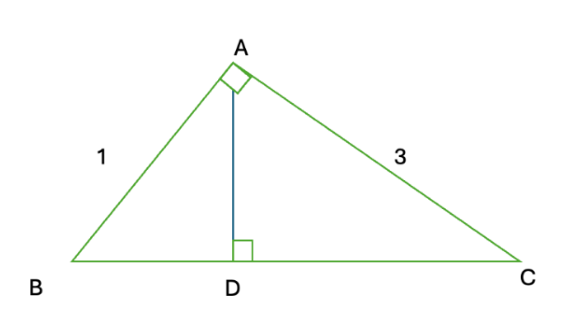
\includegraphics[width=0.35\textwidth]{images/geometry-triangles-01.png}
  \end{center}
}{
  9
}